\begin{frame}{4. Evaluation}
  \framesubtitle{4.1 Application Benchmark}

  \begin{itemize}
    \setlength{\itemsep}{10pt}
  \item \textbf{Numerical Differentiation} for experimental data
    \begin{itemize}
    \item 1D stencil computation, sensitive to computation accuracy
    \end{itemize}
  \item \textbf{Black Scholes} for finite difference option pricing
    \begin{itemize}
    \item 1D stencil, multiple time steps, requires DRAM
    \end{itemize}
  \item \textbf{Reverse Time Migration} for seismic imaging
    \begin{itemize}
    \item 3D stencil, design parallelism, operator tuning
    \end{itemize}
  \item \textbf{Bitonic Network} for high-throughput sorting
    \begin{itemize}
    \item recursive definition, design parametrisation
    \end{itemize}
  \item \textbf{Add Prediction} for Bing's sponsored search
    \begin{itemize}
    \item arithmetic intensive kernel
    \item requires effective tuning to achieve timing closure
    \end{itemize}
  \end{itemize}
\end{frame}

\begin{frame}{4. Evaluation}
  \framesubtitle{4.2 Reverse Time Migration}
  \begin{itemize}
  \item seismic imaging application for oil and gas exploration
  \item 3 dataflow kernels
    \begin{itemize}
    \item RTM -- compute intensive, multiple configurations
    \item CmdWrite -- memory write command generator
    \item CmdRead -- memory read command generator
    \end{itemize}
  \item computationally demanding
  \item use run-time reconfiguration to improve performance and efficiency
  \end{itemize}
\end{frame}


\begin{frame}{4. Evaluation}
  \framesubtitle{4.3 RTM Design Space Exploration}
  \begin{figure}[!h]
    \centering
    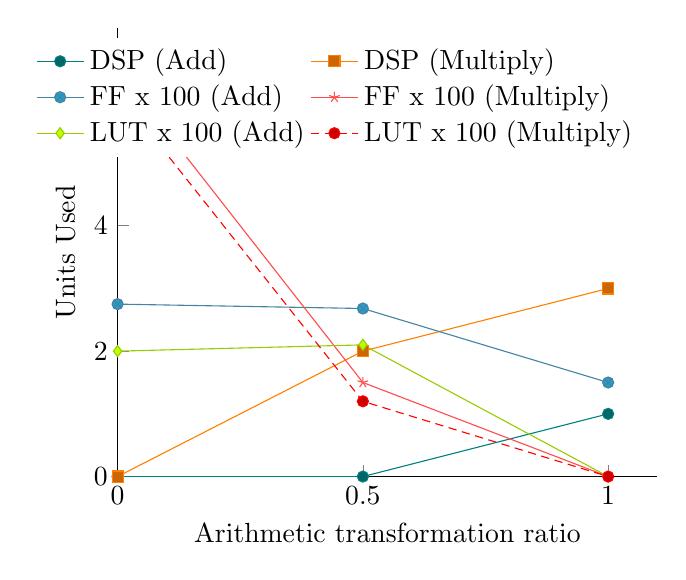
\begin{tikzpicture}
      \begin{axis}[
        cycle list name=exotic,
        xmin=0,
        ymin=0,
        axis y line*=left,
        axis x line* =bottom,
        xlabel=Arithmetic transformation ratio,
        ylabel=Units Used,
        xtick={0, 0.5, 1},
        legend columns=2,
        legend entries={
          DSP (Add),
          DSP (Multiply),
          FF x 100 (Add),
          FF x 100 (Multiply),
          LUT x 100 (Add),
          LUT x 100 (Multiply),
        },
        legend style={
          draw=none,
          cells={anchor=west}
        }
        ]
        \addplot coordinates {
          (0, 0)
          (0.5, 0)
          (1, 1)
        };
        \addplot coordinates {
          (0, 0)
          (0.5, 2)
          (1, 3)
        };
        \addplot coordinates {
          (0, 2.75)
          (0.5, 2.68)
          (1, 1.50)
        };
        \addplot coordinates {
          (0, 6.5)
          (0.5, 1.5)
          (1, 0)
        };
        \addplot coordinates {
          (0, 2)
          (0.5, 2.1)
          (1, 0)
        };
        \addplot coordinates {
          (0, 6.13)
          (0.5, 1.2)
          (1, 0)
        };
      \end{axis}
    \end{tikzpicture}
  \end{figure}
\end{frame}

\begin{frame}{4. Evaluation}
  \framesubtitle{4.4 RTM Word Length Exploration}
  \begin{figure}
    \centering
    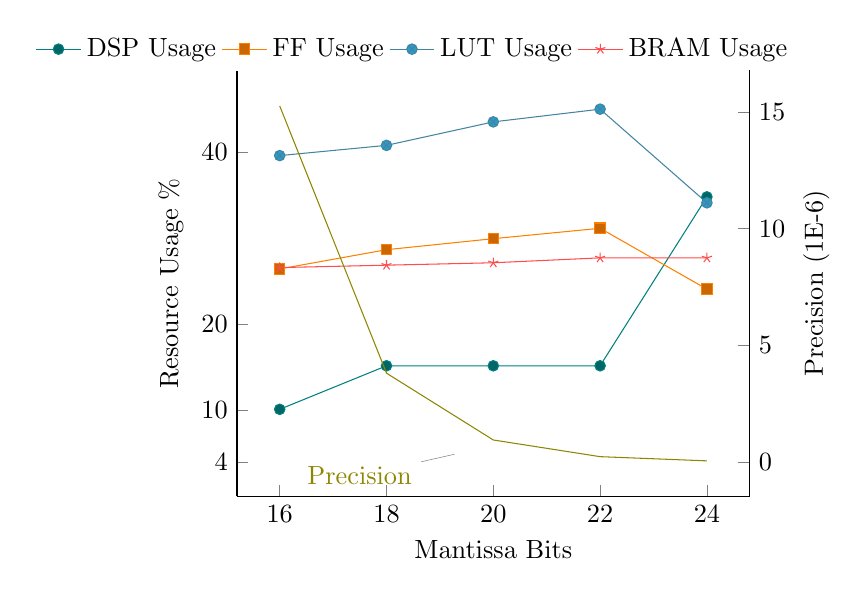
\begin{tikzpicture}[scale=0.95]
      \begin{axis}[
        cycle list name=exotic,
        ymin=0,
        axis y line*=left,
        axis x line*=bottom,
        xlabel=Mantissa Bits,
        ylabel=Resource Usage \%,
        xtick=data,
        ytick={4, 10, 20, 40, 50, 70, 80, 100},
        legend columns=4,
        legend entries={
          DSP Usage,
          FF Usage,
          LUT Usage,
          BRAM Usage},
        legend style={
          draw=none,
          anchor=east,
          at={(1.1, 1.05)}
        }
        ]
        \addplot coordinates {
          (24, 34.82)
          (22, 15.18)
          (20, 15.18)
          (18, 15.18)
          (16, 10.12)
        };
        \addplot coordinates {
          (24, 24.09)
          (22, 31.17)
          (20, 29.96)
          (18, 28.68)
          (16, 26.44)
        };
        \addplot coordinates {
          (24, 34.13)
          (22, 45.02)
          (20, 43.54)
          (18, 40.81)
          (16, 39.62)
        };
        \addplot coordinates {
          (24, 27.73)
          (22, 27.73)
          (20, 27.16)
          (18, 26.88)
          (16, 26.60)
        };
      \end{axis}
      \begin{axis}[
        ylabel=Precision (1E-6),
        axis y line*=right,
        axis x line=none,
        ]
        \addplot[color=olive] coordinates {
          (16, 15.2585)
          (18, 3.8146)
          (20, 0.9536)
          (22, 0.2394)
          (24, 0.0596)
        } node [pos=0.8,pin={190:Precision},inner sep=20pt] {};
      \end{axis}
    \end{tikzpicture}
  \end{figure}
\end{frame}

\begin{frame}{4. Evaluation}
  \framesubtitle{4.5  RTM Parallelism}
  \begin{figure}
    \centering
    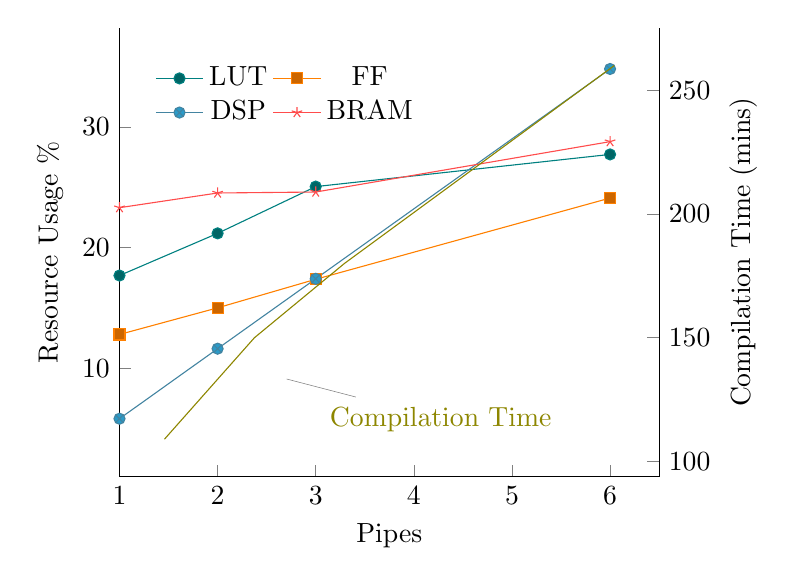
\begin{tikzpicture}
      \begin{axis}[
        cycle list name=exotic,
        xmin=1,
        ymin=1,
        xlabel=Pipes,
        ylabel=Resource Usage \%,
        axis x line* =bottom,
        axis y line* = left,
        legend columns=2,
        legend entries={
          LUT,
          FF,
          DSP,
          BRAM,
        },
        legend style={
          draw=none,
          at={(0.05,0.85) },
          anchor=west
        }
        ]
        \addplot coordinates {
          (1, 17.68)
          (2, 21.18)
          (3, 25.06)
          (6, 27.73)
        };
        \addplot coordinates {
          (1, 12.79)
          (2, 15.00)
          (3, 17.37)
          (6, 24.11)
        };
        \addplot coordinates {
          (1, 5.80)
          (2, 11.61)
          (3, 17.41)
          (6, 34.82)
        };
        \addplot coordinates {
          (1, 23.31)
          (2, 24.53)
          (3, 24.61)
          (6, 28.79)
        };
      \end{axis}
      \begin{axis}[
        ylabel=Compilation Time (mins),
        axis y line*=right,
        axis x line=none,
        ]
        \addplot[color=olive] coordinates {
          (1, 109)
          (2, 150)
          (3, 180)
          (6, 260)
        }  node [pos=0.2,pin={340:Compilation Time},inner sep=20pt] {};
      \end{axis}
    \end{tikzpicture}
  \end{figure}

\end{frame}

\begin{frame}{4. Evaluation}
  \framesubtitle{4.6 RTM Performance}

  {\small
    \begin{table}
      \renewcommand{\arraystretch}{1.4}
      \begin{tabular}{c|c|c|p{1cm}|p{1cm}|p{1cm}|p{1cm}}
                   & \textbf{CPU} & \textbf{GPU} & \textbf{FPGA S (M)} & \textbf{FPGA S (A)} & \textbf{FPGA D (M)} & \textbf{FPGA D (A)} \\
        \hline \hline
        Freq.(GHz) & 2.7          & 1.15         & 0.1                 & 0.1                 & 0.1                 & 0.1                 \\
        Time (s)   & 1458         & 52           & 18                  & 18.3                & 13.4                & 13.6                \\
        GFLOP/s    & 0.9          & 51.2         & 68.0                & 66.8                & 91.6                & 90.2              \\
        Speed-up   & 1x           & 56.8X        & 76.4X               & \textbf{74.22X}              & 102.9X              & \textbf{101.3X}              \\
        Power (W)  & 185          & n / a        & 129                 & 126                 & 128                 & 125                 \\
        Efficiency & 4.9          & n / a        & 527.1               & 527.7               & 715.6               & 721.6               \\
        Eff. Gains & 1X           & n / a        & 107.5X              & \textbf{107.0X}              & 146.0X              & \textbf{147.1X}              \\
      \end{tabular}
    \end{table}
  }

  \begin{itemize}
  \item > 97\% performance of manual FPGA design
  \item > 99\% energy efficiency of manual FPGA design
  \item functionally identical dataflow design
  \end{itemize}
\end{frame}

\begin{frame}{4. Evaluation}
  \framesubtitle{4.7 RTM Productivity}
  Evaluation results show that aspect descriptions can effectively:
  \begin{itemize}
    \setlength{\itemsep}{10pt}
  \item \textbf{control DSP mapping} -- improved timing, reduced build time vs
    increased parallelism (when DSP bound)
  \item \textbf{control word length} -- increased accuracy vs reduced
    resource usage
  \item \textbf{reveal unintuitive results} -- 2 times more
    parallelism with small impact on accuracy by reducing mantissa
    from 24 bits to 22 bits
  \item \textbf{control design parallelism} -- explore increased
    performance vs increased compilation time; identify resource
    bottlenecks
  \end{itemize}
\end{frame}

\begin{comment}
  \begin{frame}{4. Evaluation: Reverse Time Migration}
    \begin{table}
    \end{table}
  \end{frame}
\end{comment}

\begin{frame}{4. Evaluation}
  \framesubtitle{4.8 Benchmark: LOC, Performance, Resource Results}
  Comparing manual MaxCompiler designs to FAST designs:
  {\footnotesize
    \begin{table}
      \renewcommand{\arraystretch}{1.5}
      \begin{tabular}{l|c|c|c|c}
        \textbf{Kernel} & \textbf{LOC\footnote{LOC = Lines of Code}} & \textbf{API Calls} & \textbf{Performance}              & \textbf{Resource}
        \\
        \hline\hline
        CmdRead         & 1.76               & 4.33                     & \multirow{2}{1.5cm}{$ > 75\%$}        & \multirow{6}{1.5cm}{$\approx 100\%$} \\
        CmdWrite        & 1.45               & 4.13                     &                                   &                              \\
        \cline{1-4}
        RTM             & 1.17               & 10                       & \multirow{5}{1.5cm}{$ \approx 100\%$} &                              \\
        SGSmooth        & 1.85               & 14                       &                                   &                              \\
        SGDiff         & 1.75               & 14                       &                                   &                              \\
        Black-Scholes   & 2.51               & 5.5                      &                                   &                              \\
        \cline{5-5}
        Add Prediction  & 1.67               & 16                       &                                   &    $ \approx 117 \% $                          \\
        Bitonic Sort & 1.62             & 12                    &                                   &    $ \approx 100 \% $                          \\
      \end{tabular}
    \end{table}}

\end{frame}